%%
%%  chapter06.tex - Obstacle Detection and Planning for Autonomous Vehicles based on Computer Vision Techniques
%%
%%  Copyright 2014 Néstor Morales <nestor@isaatc.ull.es>
%%
%%  This work is licensed under a Creative Commons Attribution 4.0 International License.
%%

\graphicspath{{./images/chapter06/bmps/}{./images/chapter06/vects/}{./images/chapter06/}}

\chapter{Global Planning}\label{ch:chapter06}

Until now, we have seen methods oriented to the detection and, eventually, tracking of objects based on computer vision. However, we still need a strategy that allows an intelligent response when an obstacle is found, while being able to efficiently reach a given point in the map. For this purpose, we implemented a planning schema that, given a map, a localization and information about the obstacles in the neighborhood, will allow us to reach a given target safe and efficiently. We divided this schema into global planning, which will be explained in this chapter; and local planning, explained in chapter \ref{ch:chapter07}.

In the global planning level, given a goal, the algorithm is able to generate a trajectory, which will be then followed by the local planner. Despite of the fact that this level is aimed to perform a background planning in which we do not need to react to the dynamic obstacles, we have implemented our method in such a way in which it would be able to modify its trajectory if a dynamic obstacle intercepts it.

The method we designed for this task uses a \ac{MSVM} for the generation of smooth, safe and short paths. Several approaches have been made in this sense, as those shown in section \ref{ch:chapter00_02_06}, but as far as we are concerned this is the first time that Multiclass \acs{SVM} are used. The idea is that for each class (corresponding to an obstacle in the map), we train a \ac{SVM} so we can use the decision boundary as a path that can be followed to avoid the obstacle. By repeating the same process for all objects, we will get all the paths capable of avoiding an obstacle, which will be crossed with other paths in certain points. Using these points as nodes, it is possible to create a graph which can be used to find a fast way between any two points in the map. Sometimes, some boundaries do not cross each other, even where the area between them is clear. To solve this problem, we use a \ac{RNG}, with the consideration that edges will be only added if they are far enough to an obstacle.

In general, the main advantages of using \ac{SVM}  are listed in \cite{miura2006support}:

\begin{enumerate}
\item With \ac{SVM}, it is possible to generate non-linear hyperplanes which limit areas in the ground, allowing the generation of smooth paths.
\item Margin maximization allows performing a safe search strategy, ensuring that the path will always be at a certain distance the obstacles.
\item By using \acp{SVM}, the uncertainty due to the errors introduced by sensors is reduced, since they try to maximize the distance to the points that define different obstacles. If it is not possible to define a line that clearly divides two different regions, a function that tries to minimize this effect is generated.
\end{enumerate}

In addition to these features, the use of \acl{MSVM} adds another advantage.  By using them, \emph{all} possible routes in a map can be generated ensuring that they will be safe (the distance to the obstacles will be optimal) and smooth.

The method has been implemented and the code\footnote{\url{https://github.com/nestormh/svm_path_planner}}, as well as a set of videos (\url{http://youtu.be/f-tdMnHPhM8}, \url{http://youtu.be/qyqLH1huePw}) showing the performance of the algorithm and some comparisons with other methods, are available. In our implementation, we have developed a set of subroutines based on \acs{CUDA} libraries\footnote{\url{http://www.nvidia.com}}. This allowed us taking advantage of the parallel processing capabilities of the \ac{GPU}, being able to achieve a good performance without the need of expensive hardware.

\section{Method}\label{ch:chapter06_01}

For optimization purposes, the method shows two different behaviors depending on if it is the first execution or not. In the first execution, an initial map of the world is created, as well as the associated initial graph. This map can have a lower resolution than that to be used in successive iterations, as we do not need so much precision in areas far away from the current robot position. In successive executions, the graph will be extended depending on the obstacles found by the robot.

In figure \ref{fig:cp06_pipeline}, the pipeline followed by the method described in this chapter is represented. There, we distinguish between initial execution and successive iterations. In the first execution, we define the base graph, which is based just on the static obstacles shown in the map. Later, graph is updated with the obstacles and the vehicle itself. The graph generation process is composed by a clustering and obstacle inflation process, from which a set of labeled points corresponding to the contour of the safe area around obstacles are obtained. Then, we train a Multiclass \ac{SVM}, from which we will extract the decision boundaries, that will be used for the construction of the decision graph. From it, we will get the final path using graph based techniques.

\begin{figure}[h!]
      \centering
      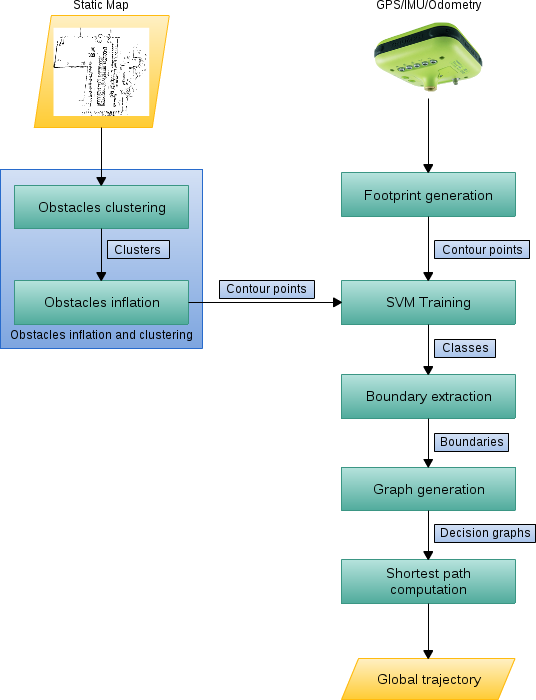
\includegraphics[width=\textwidth, height=\textwidth]{pipeline}
      \caption{ Pipeline followed in the method described in this chapter. }      
      \label{fig:cp06_pipeline}
\end{figure}

In successive iterations, obstacles and the footprint of the vehicle itself will generate a new set of contour points that will be added to the input of the \ac{MSVM}. By doing this, we just compute the boundaries for affected obstacles, avoiding to repeat the whole process for all the map.

\subsection{First execution}\label{ch:chapter06_01_01}

The generation of the initial graph is composed by the following steps:

\begin{figure}[h!]
  \centering
  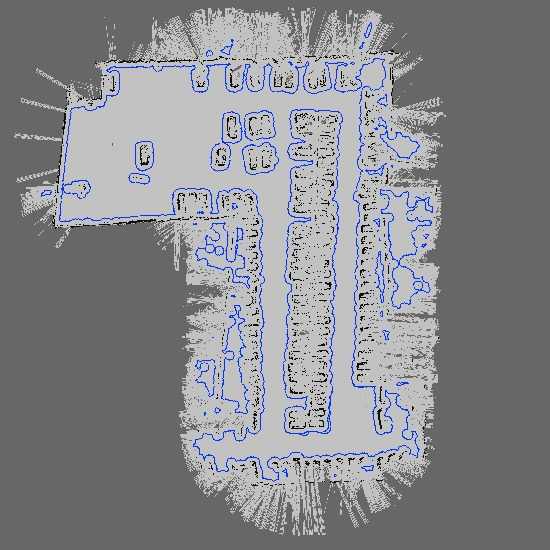
\includegraphics[width=\textwidth, height=0.75\textwidth]{figure1}
  \caption{Obstacles inflation.}
  \label{fig:cp06_obst_inflation}
\end{figure}    

\subsubsection{Obstacles Inflation}\label{ch:chapter06_01_01_01}

In our implementation, we have considered the world map as a grid of a certain resolution in which obstacles are represented using a values from 0 to 255, where 0 represents a free area and 255 is an obstacle. This costmap is better explained in section \ref{ch:chapter07_01_01}, in the next chapter. Using this map, we calculate the cost for each cell $c(x,y)$ of the map using the following function:

\begin{equation}\label{eq:cp06_cell_cost}
 cost(c) = 253 * \exp( -1 \cdot \beta \cdot (\| nearest(c) - c\| - \rho) )
\end{equation}

, where $\beta$ is a scaling factor that increases/decreases the slope of the cost function, $nearest(c)$ is the position of the nearest cell in the map to the cell $c$ marked as obstacle, and $\rho$ is the circumscribed radius of the robot. The function is scaled to $253$ as 254 and 255 are reserved values. Based on the cost map generated, we mark all values over a threshold $\tau$ as obstacle, so the cost map becomes a binary matrix. From this matrix we extract the boundaries using the method in \cite{suzuki1985topological}. In figure \ref{fig:cp06_obst_inflation}, the output after doing this step is shown.


\subsubsection{Obstacles Clustering}\label{ch:chapter06_01_01_02}

The boundaries obtained in the previous step are used as input for the obstacles clustering stage. At this point, we have a cloud of points $\mathcal{P}$ from which we do not know if they belong to the same obstacle or not. This clustering is done using the method described in \cite{rusu2009semantic}. The procedure is described at algorithm \ref{alg:obstacles_clustering}.

\begin{algorithm}[h!]
\caption{Obstacles clustering}
\label{alg:obstacles_clustering}
\begin{algorithmic}
\ForAll{$p_i \in \mathcal{P}$}
  \State add $p_i$ to the queue $\mathcal{Q}$.
  \ForAll{$p_i \in \mathcal{Q}$}
    \State look for the set of neighbors of $p_i$, $\mathcal{P}_i^k$, inside a circle of radius $d_{obst}$.
    \ForAll{$p_i^k \in \mathcal{P}_i^k$}
      \If{\textbf{not} $p_i^k$ is processed}
	\State add $p_i^k$ to $\mathcal{Q}$.
      \EndIf
    \EndFor
    \If {all points in $\mathcal{Q}$ have been processed} 
      \State add $\mathcal{Q}$ to the list of clusters $\mathcal{C}$.
      \State reset $\mathcal{Q}$ to an empty list.
    \EndIf
  \EndFor
\EndFor
\end{algorithmic}
\end{algorithm}

In this algorithm, $d_{obst}$ is the maximal distance between a pair of points to consider them to belong to different obstacles.

\subsubsection{\ac{SVM} Training}\label{ch:chapter06_01_01_03}

Once we have clustered the inflated obstacles into different objects, we want to know which is the best path between them in terms of distance to the obstacles and smoothness. The way in which this is done makes the difference with respect to other \ac{SVM} based path planning algorithms. Unlike the methods seen at the Introduction of this thesis (section \ref{ch:chapter00_02_06}), our method uses a Multiclass \acs{SVM} in order to obtain the best path between the obstacles. In general, in classification, generation of a solution for the multiclass classification in a single step is usually avoided. Instead of this, a combination of several binary \ac{SVM} classifiers is used. The most known methods for doing that, based on the review in \cite{hsu2002comparison, duan2005best}, are:

\begin{itemize}
 \item One-versus all using winner-takes-all.
 \item One-versus-one using max-wins voting.
 \item Directed Acyclic Graph SVM (DAGSVM).
\end{itemize}

In our implementation we used a one-versus-all strategy. That is, for each set of points $C_i$ corresponding to a cluster in the set of clusters $\mathcal{C}$, we create two classes, one formed by the point set $C_i$, and the other composed by the points belonging to the remaining clusters $\{\mathcal{C} - C_i\}$. From these two classes, we train a single \ac{SVM}, which will give us the parameters $\alpha_k$ corresponding to the support vectors $x_k$ and their labels $y_k$, which will be later used by the equation \ref{eq:appendixSVM_soft_discriminative_function}. In our implementation, we used a \acs{GPU} based implementation of the \ac{SVM}, described in \cite{athanasopoulos2011gpu}. The use of this implementation improved notably the time required by our implementation for the \ac{SVM} training step.

\subsubsection{Boundary extraction}\label{ch:chapter06_01_01_04}

Once we have obtained the parameters $\alpha_k$, $x_k$ and $y_k$, we need to know where the decision boundary is for each class. That is, based on the equation \ref{eq:appendixSVM_soft_discriminative_function}, we look for the $x$ points that satisfy:

\begin{equation}\label{eq:cp06_decision_boundary}
 y = \sum_{k \in S} \alpha_k y_k K(x_k, x) + b = 0
\end{equation}

These points will allow us obtaining a non-linear decision curve. In figure \ref{fig:cp06_decision_boundary_3d}, we have represented, for each cell $(x,y)$ in a map, the values obtained from equation \ref{eq:cp06_decision_boundary} as their $Z$ coordinate, using the parameters obtained after training a given class. The plane represented in black is $Z=0$, so all cells in which this plane intersects with the named function will belong to a path.
In fact, as solving the equation \ref{eq:cp06_decision_boundary} can be too computationally expensive, we have optimized the implementation of this step as follows: First, we sample the map into a grid of a given resolution. For each cell in the map, we obtain the value given by equation \ref{eq:cp06_decision_boundary}. If positive, we assign $1$ to this cell. Else, we assign $0$. This process is executed over the \ac{GPU} using a \ac{CUDA} function developed for this purpose, so it is fully parallelized, taking a very small amount of time to check all the cells, obtaining even better times than in, for example, other \ac{DP} based approaches.

\begin{figure}[h!]
  \centering
  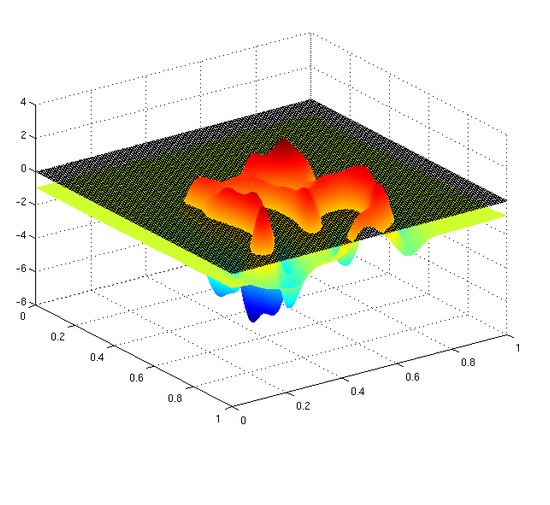
\includegraphics[width=\textwidth, trim=0 0 0 0,clip]{figure2}
  \caption{Output of \ref{eq:appendixSVM_soft_discriminative_function} for a given class.}
  \label{fig:cp06_decision_boundary_3d}
\end{figure}

Once we created the new map, we extract the decision boundaries. Points are stored in the point set $\mathcal{B}$, which will be shared by all classes. At this point we do not store neighborhood information, but we add to each point $p_i$ a label $l_i$, in order to know the class from which they were initially generated. This information will be used in the graph generation stage.

\subsubsection{Graph generation}\label{ch:chapter06_01_01_05}

The graph generation stage takes as input the points in $\mathcal{B}$ and tries to generate a connectivity graph that will be used later to obtain the shortest paths between points pairs in the map. At a first glance, we could just connect all the points generated by the same class , and join those subgraphs by the points in which the decision boundaries cross each other. Unfortunately, we can not do that because there are situations where there is a big free of obstacles area, which avoids the connections between two classes, making it impossible to travel from the path belonging to one class to the other. This effect can be observed for some of the obstacles represented in figure \ref{fig:cp06_nng}.
To solve this problem, in our method we propose a combination of a \acf{RNG} based on the Delaunay triangulation \citep{lingas1994linear}, and a \acf{NNG} \citep{eppstein1997nearest}.

\paragraph{\acf{NNG}}\label{ch:chapter06_01_01_05_01}

In order to obtain the \ac{NNG}, we calculate a $kd-tree$ for the points in $\mathcal{B}$. For each point in $\mathcal{B}$, we look for the neighbors inside a given radius circle. If there are not obstacles between the point $u$ and a certain neighbor $v$, an edge $e(u,v)$ is added to the graph. By doing this, we allow the robot to go from the path obtained from a class to another if points are close enough and there are not obstacles in the neighborhood. In figure \ref{fig:cp06_nng}, we can see the graph as it would look like at this point of the execution. As can be seen, there are some boundaries that are not connected, despite that there is a free area between them. This problem is solved with the \acf{RNG}.

\begin{figure}[h!]
  \centering
  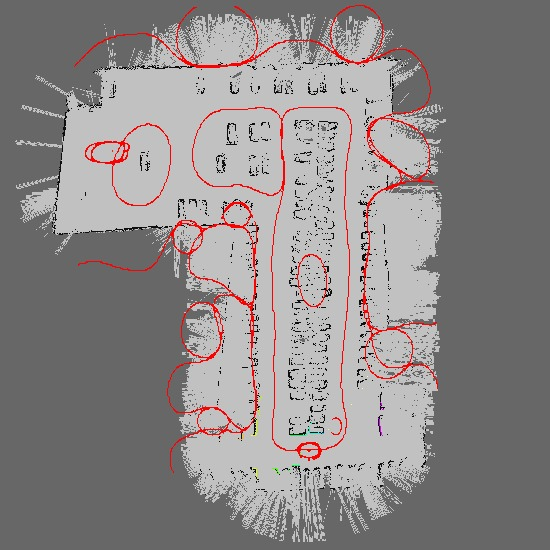
\includegraphics[width=\textwidth, height=0.75\textwidth]{figure3}
  \caption{\acf{NNG}.}
  \label{fig:cp06_nng}
\end{figure}

\paragraph{\acf{RNG}}\label{ch:chapter06_01_01_05_02}

For the generation of the \ac{RNG}, we use the set of labels $l_i \in \mathcal{L}$ described in section \ref{ch:chapter06_01_01_04}. First, we obtain the Delaunay Triangulation \citep{su1997comparison} using the points in $\mathcal{B}$ as input. In our implementation, we used the method in \cite{rong2008computing} for that. Then, we iterate through the edges $e(u,v)$ of the triangles. For each one of these edges, we check that there are not obstacles between $u$ and $v$. If this condition is true, and $l_u \neq l_v$, the edge $e$ is added to our graph. In our implementation, we process all edges simultaneously over the \acs{GPU}, saving a lot of time. Edges obtained by the \ac{NNG} are tested, too. The obtained graph is depicted in figure \ref{fig:cp06_rng}.

\begin{figure}[h!]
  \centering
  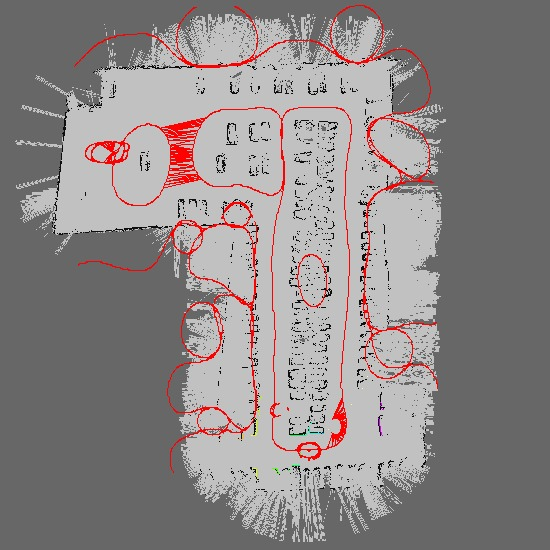
\includegraphics[width=\textwidth, height=0.75\textwidth]{figure4}
  \caption{\acf{RNG}.}
  \label{fig:cp06_rng}
\end{figure}%

At this point, we have a graph that allows us going from any point in the map to another ensuring a safe and smooth path. However, in successive iterations, there could be obstacles that were not there when the initial map was created, so the graph must be updated in the following executions. The process that solves this situation is explained in the following section.

\subsection{Successive executions}\label{ch:chapter06_01_02}

The steps in the successive executions are quite similar to those in the initial execution. However, for optimization purposes, we do not need to recalculate the whole map in each execution, but extend the map we had from the previous one. The steps needed are the following:

\subsubsection{Obstacles Inflation and clustering}\label{ch:chapter06_01_02_01}

This step is similar to that described in section \ref{ch:chapter06_01_01_01}. The only difference is that points from the inflation boundary are compared to those in the original map. To do that, we calculate a $kd-tree$ from the set of points obtained in the first execution, $\mathcal{O}_{old}$. Then, for each point $o_i$ in the new set, $\mathcal{O}_{new}$, we look for the nearest point in $\mathcal{O}_{new}$. If the nearest point of $o_i$ is nearer than a given threshold, it is removed from $\mathcal{O}_{new}$. Then, the clustering step is performed similarly as happened in the first execution, but with the filtered set $\mathcal{O}_{new}$.

\subsubsection{Footprint generation}\label{ch:chapter06_01_02_02}

We want to get the path starting from an initial point (which coincides with the current position of the robot in the map) towards to a goal. To do this, we need to add a pair of fake obstacles that help to generate the trajectory the robot will follow from its current position towards the nearest point in the graph, and from the graph to the goal. These fake obstacles will also prevent the robot from starting the trajectory in an impossible angle given its current orientation. Same applies for the desired goal position and orientation. Before starting all the process, we check that we are not currently in a collision with an obstacle. In this case, the process is aborted and recovery behaviors should be triggered. If everything is right, we generate a set of points ($\mathcal{F}_L$) that go from the position $A(-\rho, +\rho)$ to the position $B(\rho, \rho)$, and another one ($\mathcal{F}_R$) coming from $C(-\rho, -\rho)$ to $D(\rho, -\rho)$, being $\rho$ the circumscribed radius of the robot defined in section \ref{ch:chapter06_01_01_01}. 

\begin{figure}[h!]
  \centering
  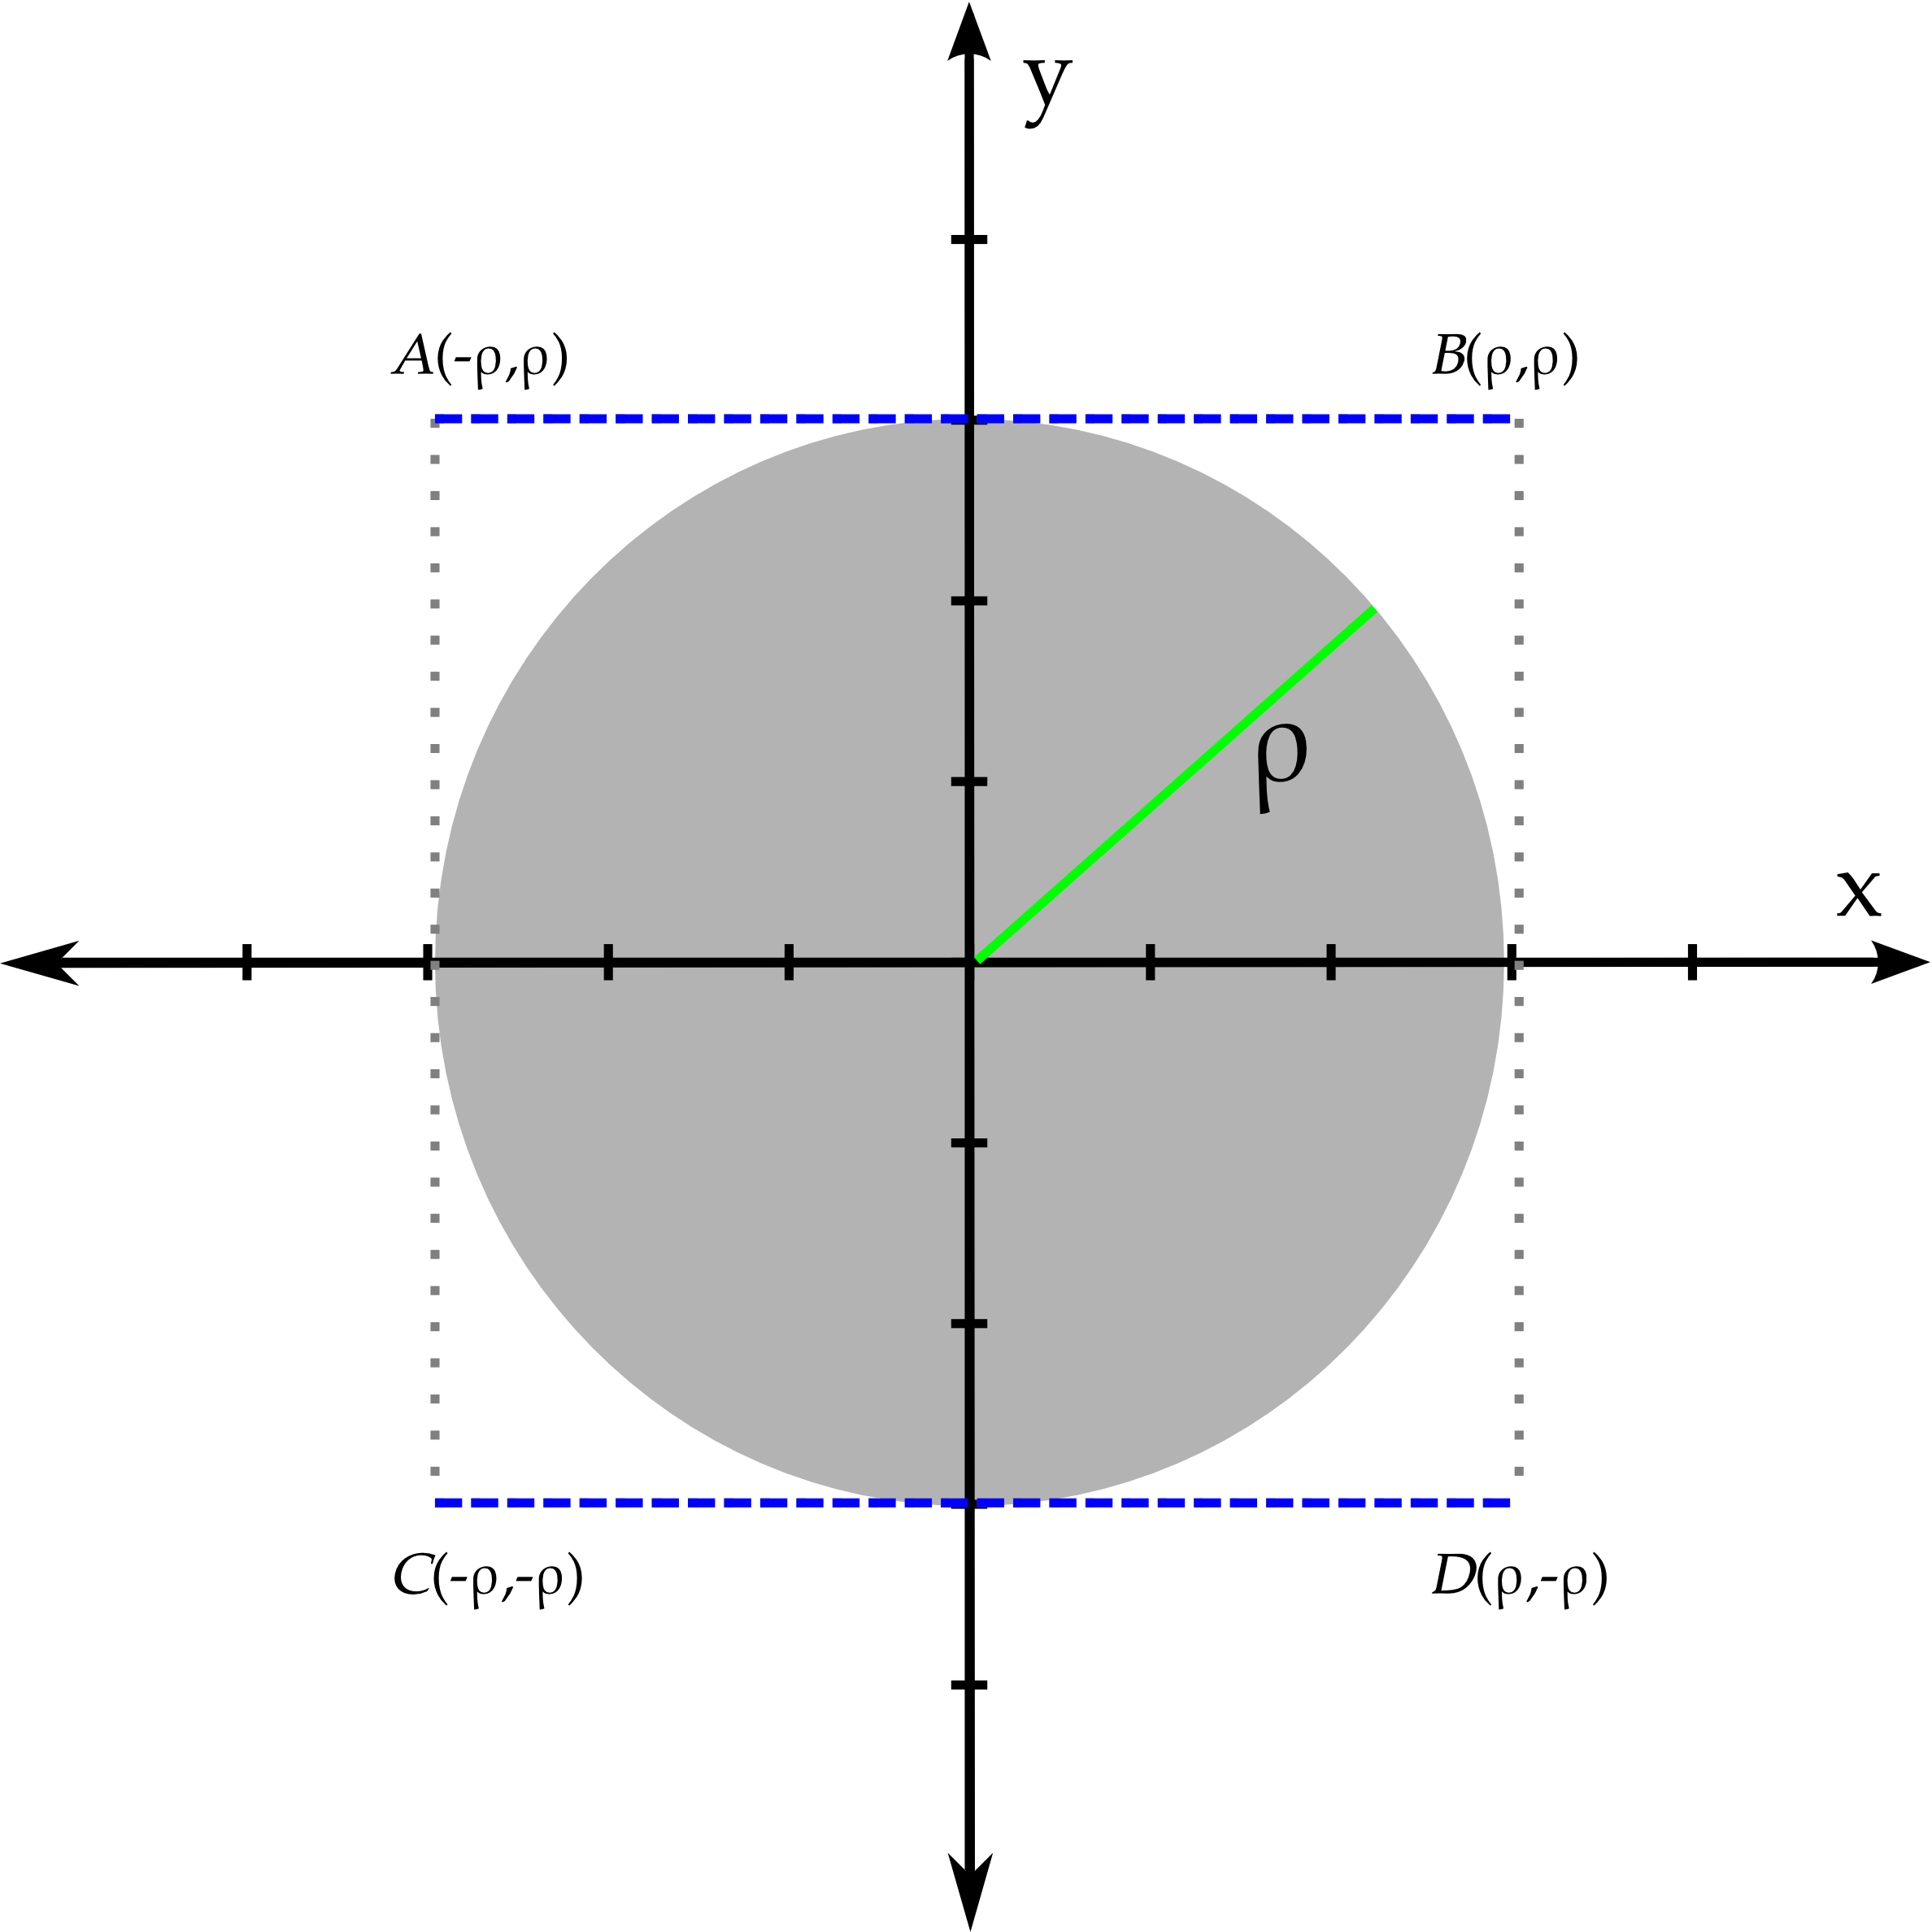
\includegraphics[width=\textwidth, trim=0 0 0 0,clip]{figure5}
  \caption{Footprint generation.}
  \label{fig:cp06_footprint_generation}
\end{figure}%

In figure \ref{fig:cp06_footprint_generation}, this process is represented, as well as points $A$, $B$, $C$ and $D$. Each point set will be considered as a class in the following. Coordinates of the obtained point sets $\mathcal{F}_L$ and $\mathcal{F}_R$ are relative to the robot position, so we must transform them to map coordinates using the transformation matrix

\begin{equation}\label{eq:cp06_Rt_footprint}
 Rt = \left ( \begin{array}{ ccc }
  \cos(\theta_s) & -\sin(\theta_s) & s_x \\
  \cos(\theta_s) & -\sin(\theta_s) & s_y \\
  0 & 0 & 1
 \end{array} \right )
\end{equation}

, where $s(x,y)$ is the starting point (the current point of the robot), and $\theta_s$ its orientation. Once we have $Rt$, each point $f_{L,i} \in \mathcal{F}_L$ is transformed so its new position $f'_{L,i}$ becomes ${f'}_{L,i}^T = Rt \cdot f_{L,i}^T$. Same applies to the points in $\mathcal{F}_R$.

The same process is performed for the goal point $g(x,y)$ and its orientation $\theta_g$. At this point, we have limited the orientation of the vehicle in the start and goal points, but not its direction. This limitation will be controlled in the process described in section \ref{ch:chapter06_01_02_04_01}. If we would have closed the obstacle by joining the points $A$ and $C$ with a new set of points, we would be in  risk of having imprecise decision boundaries, preventing us from finding a feasible path.

\subsubsection{\ac{SVM} training, boundary extraction and graph generation}\label{ch:chapter06_01_02_03}

Once we have got the classes related to the new points given by the sensors of the robot, and the four classes corresponding to the footprints, the stages of \ac{SVM} training, boundary extraction and graph generation are exactly the same described in section \ref{ch:chapter06_01_01}. The only difference is that we remove the paths that were in the original graph but that are not longer traversable due to the presence of dynamic obstacles. Anyway, as we consider that the initial iteration contains just static obstacles, the original graph is stored for its use in future executions.

\subsubsection{Shortest path calculation}\label{ch:chapter06_01_02_04}

At this point, we have a graph with all the feasible paths in the map completely updated, including the new obstacles. With this graph, it is possible to find a safe and smooth path between the given starting and goal positions and their orientations.

\paragraph{\underline{Looking for the starting and goal points into the graph:}}\label{ch:chapter06_01_02_04_01}

As said in section \ref{ch:chapter06_01_02_02}, we have limited the robot to start with a given orientation, but at this point we are still not taking its direction into account. To solve this, given the current position of the robot and the goal, $s(x,y)$ and $g(x,y)$, and their orientations, $\theta_s$ and $\theta_g$, we obtain the points

\begin{equation}\label{eq:cp06_start_goal_points}
\begin {array}{l}
 s_1 = (s_x + \rho * \cos(\theta_s), s_y + \rho * \sin(\theta_s)) \\
 g_1 = (g_x - \rho * \cos(\theta_g), g_y - \rho * \sin(\theta_g))
\end{array}
\end{equation}

Then, we use the points $s_1$ and $g_1$ to look for the nearest point in the graph, using the kd-tree previously created in the previous sections. These points, $s_2$ and $g_2$, will be the ones used by the Dijkstra shortest path algorithm to find a path. This operation is better described in figure \ref{fig:cp06_findstartgoal}. Using the current position of the robot (starting point $s$), represented in red, and its orientation, we obtain the point $s_1$ (the point in magenta) based on the equation \ref{eq:cp06_start_goal_points}. In the graph, the nearest point to $s_1$ , $s_2$ , is the initial point used by Dijkstra algorithm.

\begin{figure}[h!]
  \centering
  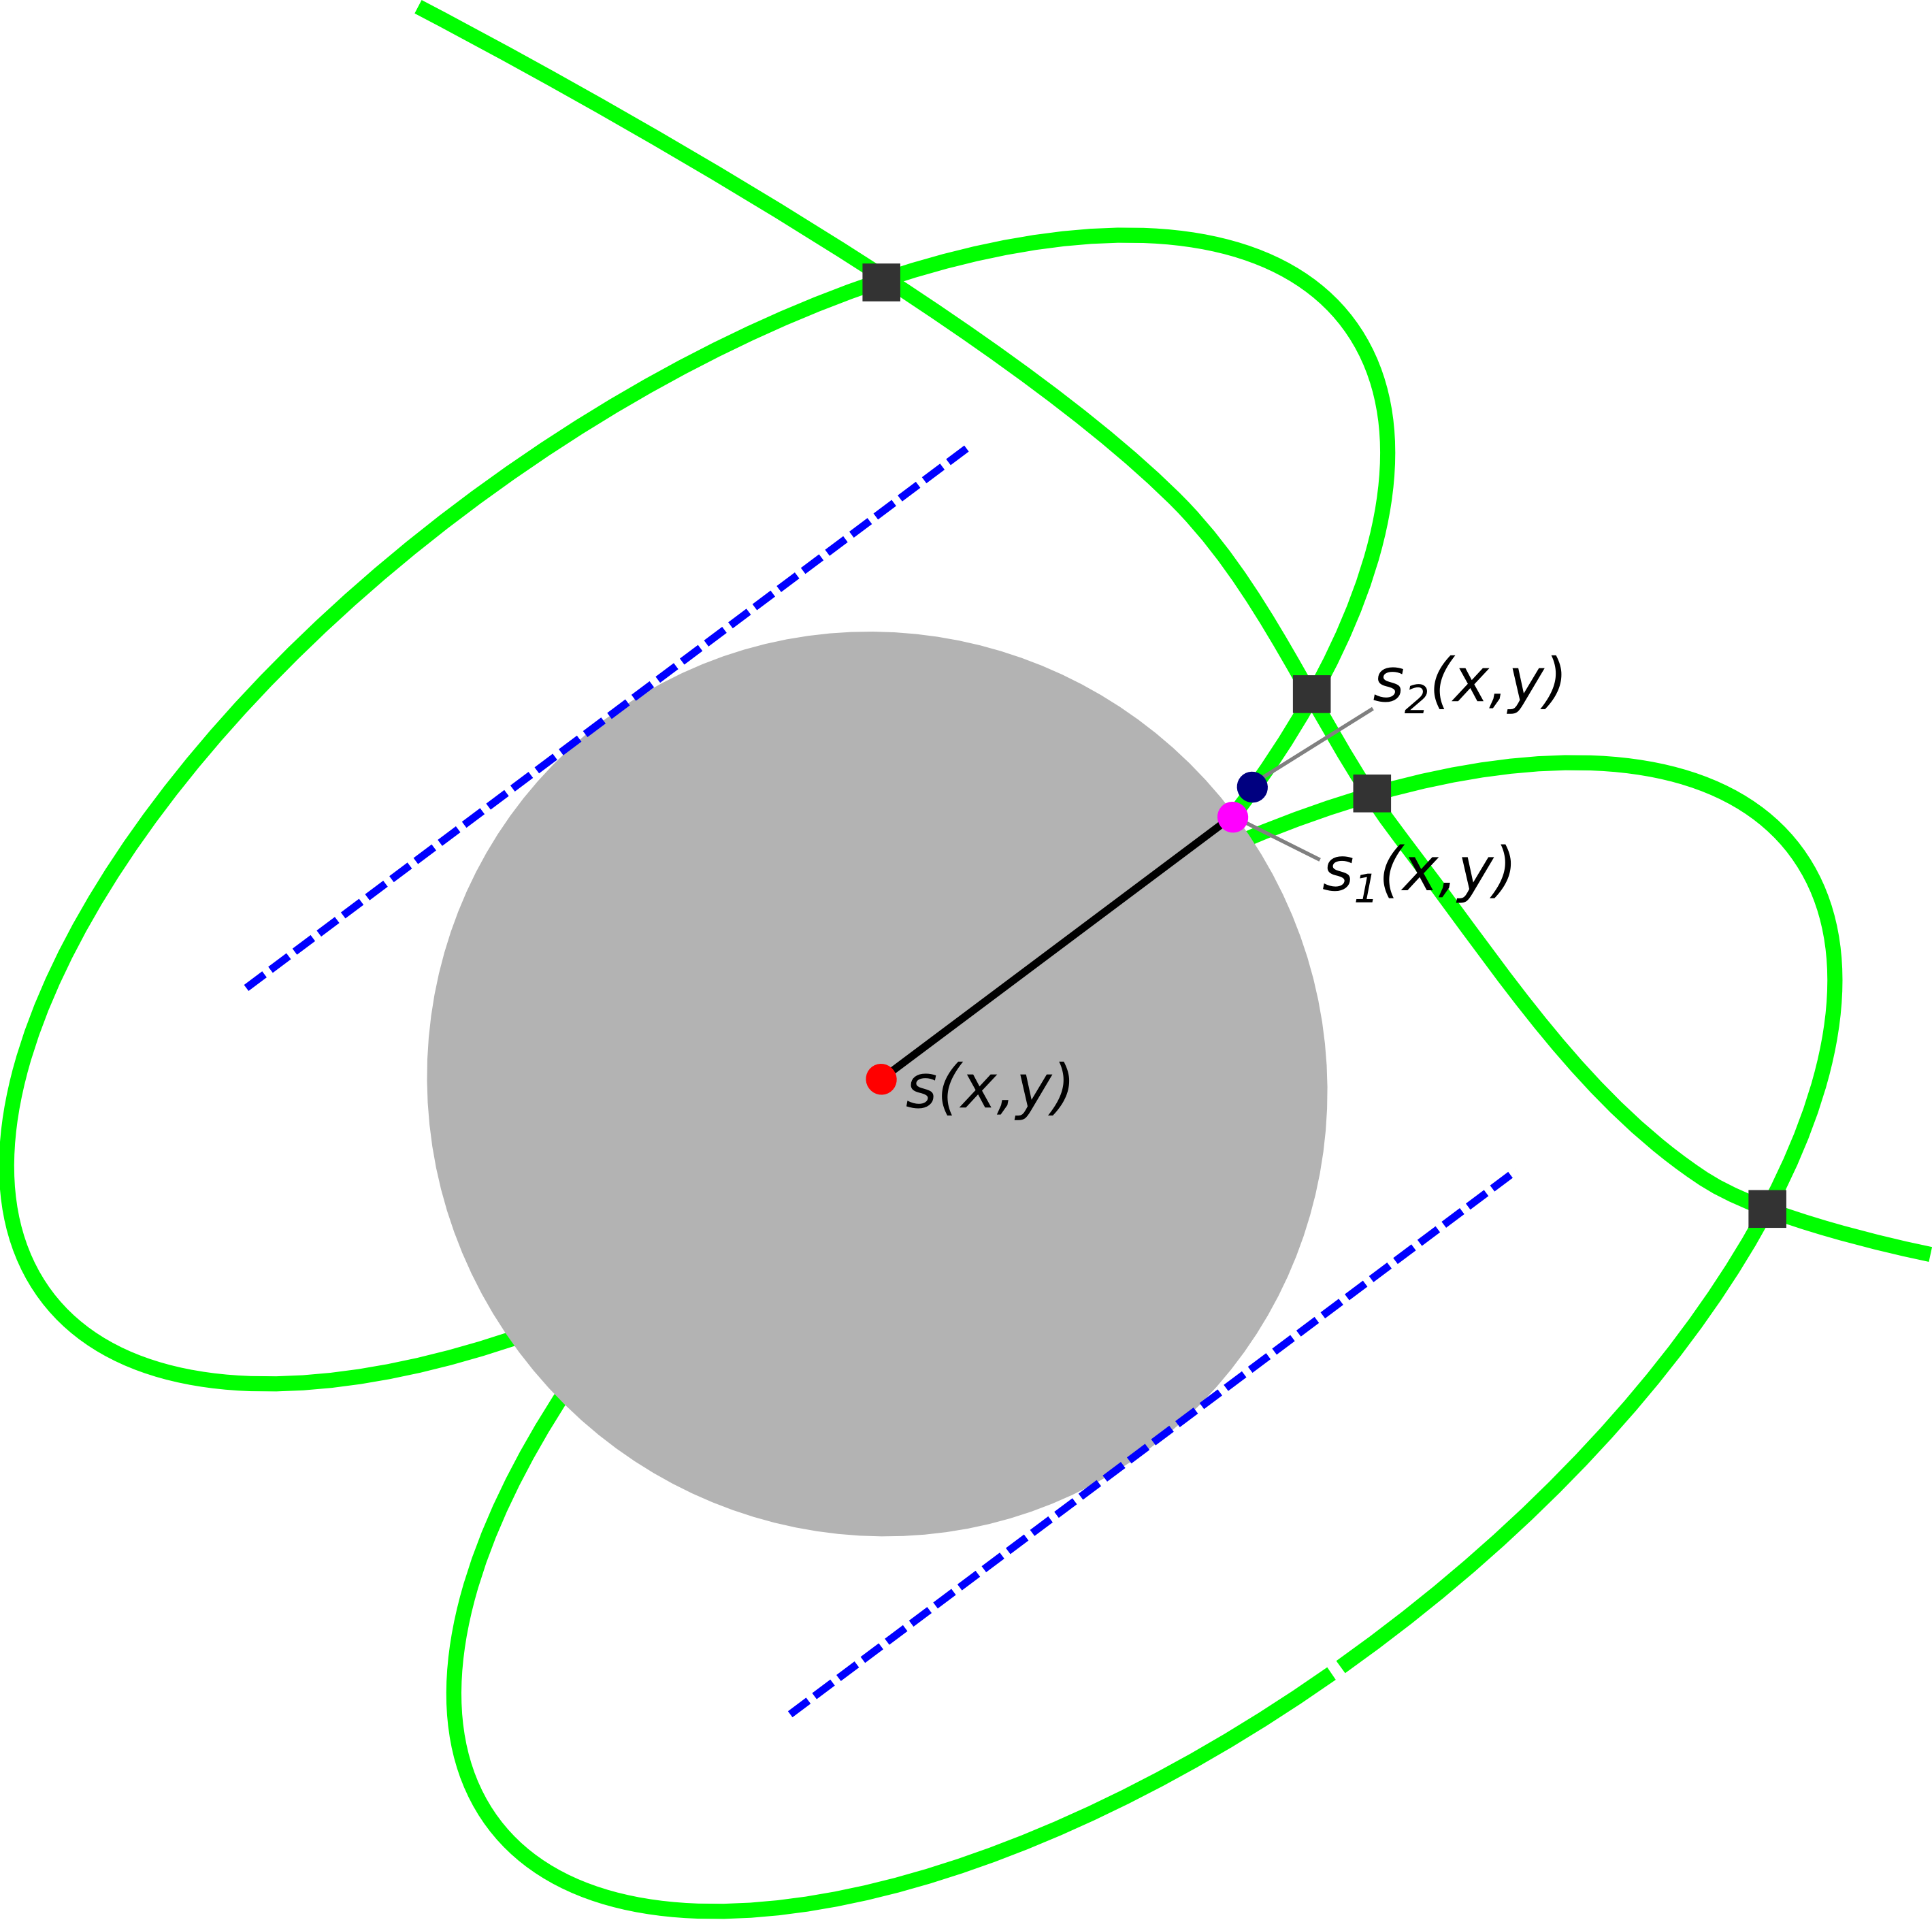
\includegraphics[width=\textwidth, trim=0 0 0 0,clip]{figure6}
  \caption{Starting and goal point selection process.}
  \label{fig:cp06_findstartgoal}
\end{figure}

\paragraph{\underline{Looking for the shortest path:}}\label{ch:chapter06_01_02_04_02}

Before applying Dijkstra, we need to know if the goal is reachable. To do that, we check the graph connectivity. If $s_2$ and $g_2$ are in the same connected component, the goal is reachable. This checking is needed because there will be a graph in every place in which there is a hole between the limits obtained in the obstacles inflation step. This is because it is faster making a connectivity checking than testing whether a graph is in a traversable area or not. We suppose that the robot will always start in a valid area.
Once we have done this verification, Dijkstra is applied and the path is obtained. Points $s$ and $g$ are added to the beginning and the end of the path. The whole implementation of the algorithm has been tested on a PC i7-3630QM with 8GB RAM and a NVIDIA GT 640M, being able to work in a real time navigation application for an autonomous robot.

Some improvements could be incorporated to the current method, like using the extended \ac{SVM} version described in \cite{qingyang2012local}, which would allow satisfying additional restrictions, such as the robot position or heading. Also, the path generated by our method could be smoothed again using a second \ac{SVM} step, as done for the path generated by the Voronoi diagrams in \cite{yang2012safe}.

In figure \ref{fig:cp06_final_path}, the final path obtained by the algorithm is shown. In chapter \ref{ch:chapter08}, some results are shown, demonstrating the good behavior of the method, comparing it with some of the best path planning algorithms based on \ac{SVM}.

\begin{figure}[h!]
  \centering
  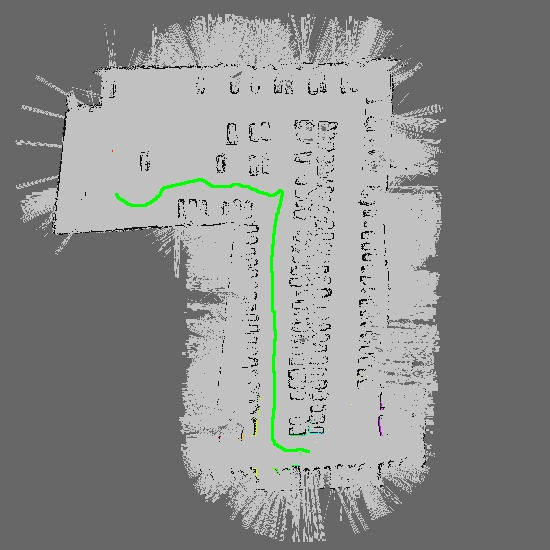
\includegraphics[width=\textwidth, height=0.75\textwidth]{figure7}
  \caption{Final path.}
  \label{fig:cp06_final_path}
\end{figure}

\section{Summary}\label{ch:chapter06_03}

In this chapter, we have shown an alternative to classical path planning methods, based on a \acf{MSVM}. Advantages of using this method as a base for our algorithm are that we can generate continuous non-linear separating surfaces between classes that, joined all together, allow the creation of a graph used for the generation of smooth, short and safe paths. The method has been developed taking advantage of the use of a \ac{GPU} in order to reduce the required computational time.

In this method, we have considered an initial graph, which is extended in the following iterations, allowing the inclusion of new obstacles and the influence of the vehicle itself in the generation of trajectories. This method was thought for an early version of the local planner described in the next chapter, in which we needed the trajectory to start just from the current position of the vehicle. However, as we will see in the next chapter, this restriction is not longer needed, since we started using other strategies based on the Frenét space, which makes things even easier.

In the future, the initial graph generation step of this method could be also a good starting point for the generation of a full \ac{RNDF} from the scratch, given an occupancy map in which an unstructured area is represented.
